%  !TeX  root  =  user_guide.tex

\section{Морфометрический анализ}\label{sec:rasterrain}

% when the revision of a section has been finalized,
% comment out the following line:
%\updatedisclaimer

Модуль морфометрического анализа  может быть использован для расчета
угла уклона, экспозиции, индекса пересечённости и общей кривизны цифровых
моделей рельефа (ЦМР). Модуль очень прост в использовании благодаря
интуитивно понятному графическому интерфейсу
(см. Рисунок~\ref{fig:raster_terrain_dialog}). Для расчета требуются
следующие параметры, которые нужно указать перед началом работы:

\begin{itemize}[label=--]
\item \textbf{Анализ}: Может быть одним из следующих: уклоны,
экспозиция, индекс пересечённости, общая кривизна.
\item \textbf{Исходный слой}: Выбирается растр из списка загруженных растровых
слоев.
\item \textbf{Выходной слой}: Задается имя и путь выходного изображения.
\item \textbf{Формат вывода}: Выбирается формат выходного растра (по
умолчанию GeoTiff).
\end{itemize}

Description of the analysis:

\begin{itemize}[label=--]
\item \textbf{Уклон}: Вычисляет угол наклона для каждой ячейки в градусах (алгоритм
основан на вычислении первой производной).
\item \textbf{Экспозиция}: Экспозиция (начиная с 0~градусов на север, против часовой стрелки).
\item \textbf{Индекс пересечённости}: Количественная оценка неоднородности рельефа.
\item \textbf{Общая кривизна}: Суммарная кривизна, включающая плановую и профильную кривизну.
\end{itemize}

\begin{figure}[ht]
   \centering
   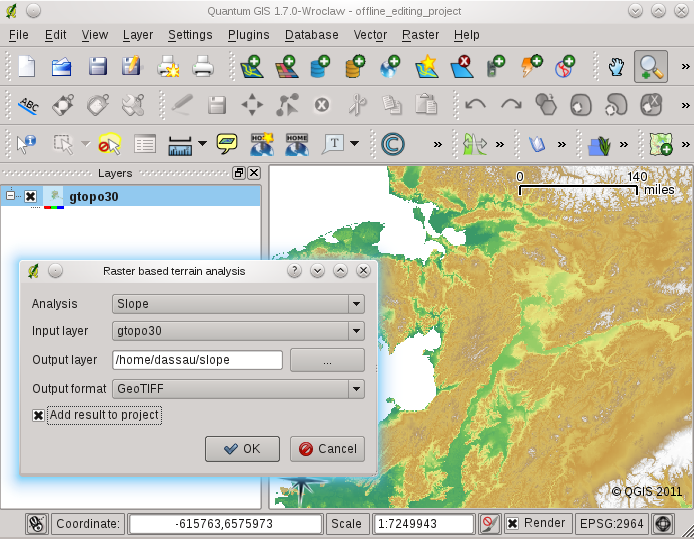
\includegraphics[clip=true, width=9cm]{raster_terrain_dialog}
   \caption{Модуль морфометрического анализа \wincaption}\label{fig:raster_terrain_dialog}
\end{figure}

\minisec{Использование модуля}\label{raster_terrain_usage}

\begin{enumerate}
  \item Запустите QGIS и загрузите растр цифровой модели рельефа.
  \item Активируйте модуль <<Морфометрический анализ>> в <<Менеджере модулей>>
  (см. Раздел~\ref{sec:load_core_plugin}) и нажмите на кнопку
  \toolbtntwo{raster_terrain}{Морфометрический анализ}, которая появилась
  на панели инструментов QGIS. Откроется окно модуля, изображенное на
  Рисунке~\ref{fig:raster_terrain_dialog}.
  \item Выберите метод анализа (например, \dropmenuopt{Уклоны}).
  \item Укажите выходной файл и его формат.
  \item Нажмите \button{Ok}.
\end{enumerate}

\FloatBarrier
